%
% Copyright (c) 1996 Bunyip Information Systems Inc.
% All rights reserved
%
% Archie 3.5
% August 1996
%
% anonftp.tex
%

\chapter{The anonymous FTP catalog}


The Archie system is designed to maintain several different information
catalogs, of various types. Nonetheless, it was originally conceived to
maintain a catalog of files available by anonymous FTP, and this is still the
application for which it most popular today.

Now that the arserver, arexchange, and arretrieve programs have been
configured (according to the instructions in ``Configuring the Basic System'' on
page~\pageref{chap:configure}), you can go about setting up the system to
maintain an anonymous FTP catalog.


\section{Overview}

In general, to set up the anonymous FTP catalog, anonftp, the following steps
must be followed:

\begin{itemize}
\item
Make sure the configuration files listed in the previous sections have been
modified to reflect your system and information retrieval needs. In
particular, make sure that the domains database has been configured (see
ardomains).

\item
 Load the Data Host information into the Host Information Files.
Use the host\_manage program to
add, delete and modify individual host entries.  This is explained below.
\end{itemize}

\section{Choosing Data Hosts to enter}

You need only enter into the Host Databases, those Data Hosts for which you
plan to be directly responsible. You need not (and should not) enter other
sites. Once you start participating in the global inter-Archie data exchanges,
those data hosts for which you are not responsible will be entered into your
database automatically. Similarly, you need not delete those sites for which
you are not responsible. The exchange subsystem will propagate this
information from the ``master'' Archie system responsible for that site.




\alertbox{In general Bunyip maintains a policy to only index Data
Hosts which are aware, and approve of the practice.}


\section{Support for ls-lR.gz}
\new

Archie can now retrieve from anonymous ftp sites pre-generated ls-lR.gz files
In order to activate this you will need to setup the file
\Path{\archie/etc/options.cf} in the following way.

\begin{center}
\begin{tabular}{l}
\Param{\#} \\
\Param{\#TYPE           NAME                    PATH} \\
\Param{\#} \\
\Param{\#} \\
\Param{COMPRESS       GZIP                    /usr/local/bin/gzip} \\
\Param{UNCOMPRESS     GZIP                    /usr/local/bin/gunzip} \\
\end{tabular}
\end{center}

Where \Path{/usr/local/bin/gzip} is where the program \Path{gzip} is located on
your system.

You also need to fix the file \Path{\archie/etc/arretdefs.cf} by replacing
the line

\param{anonftp:unix\_bsd:image:.Z:anonymous:::-R:*?:ls-lR}

by 

\param{anonftp:unix\_bsd:image:.gz,.Z:anonymous:::-R:*?:ls-lR}



Hence when using the \Param{-Z} option in  retrieve mode 

\comm{arcontrol -r -Z}

Archie will try to first locate the ls-lR.gz file. If it can't it will
look for ls-lR.Z, ls-lR in that order and as a last resort
dynamically create the new listing.

\section{Adding sites}

\alertbox{You may want to start by entering one site into the Host Database
(using host\_manage) then testing the system before entering more sites. Once
entered, you can manually run arretrieve, and arcontrol in its various modes
(retrieve, parse and update) to get a feel for how the system operates.}




\section{Parser failures}

\begin{figure}
\begin{center}
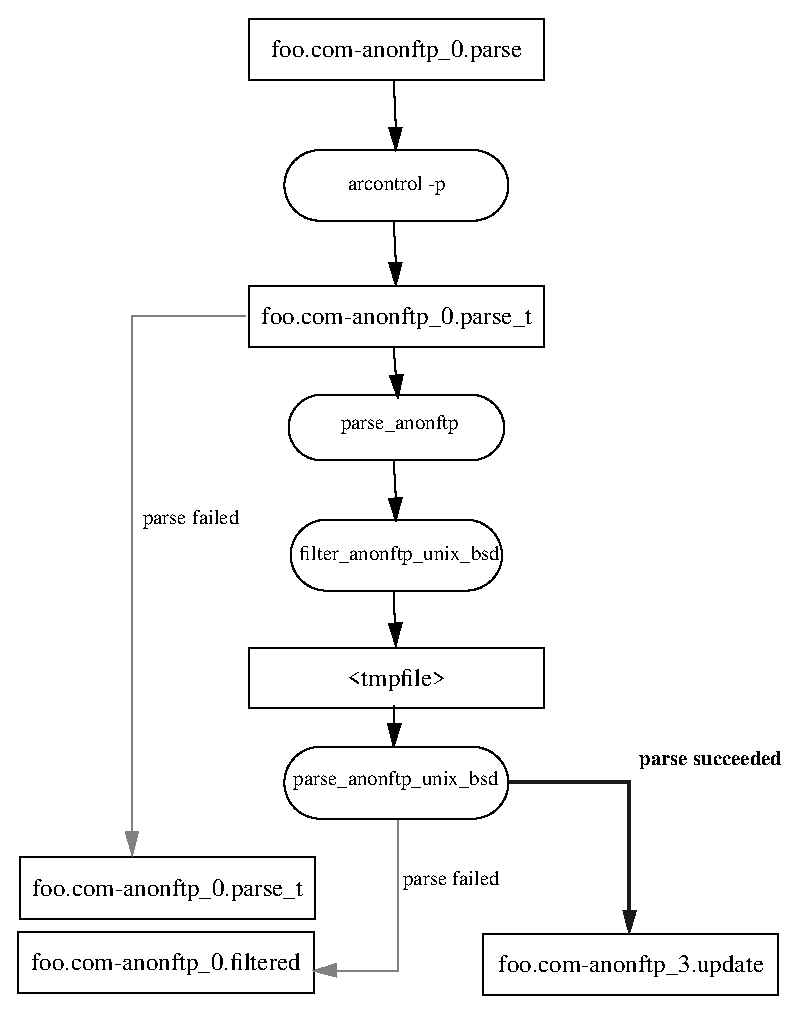
\epsfig{file=figs/parse.eps}
\end{center}
\caption{The parsing process}
\end{figure}


When the parsing phase of the anonftp catalog fails on a particular data host
the temporary parse file (with the parse\_t suffix) is not removed from the
holding directory (\Path{\archie/db/tmp}). In addition, the filtered file is renamed
with the suffix .filtered to allow the system administrator to see both the
unfiltered and filtered versions. The system administrator may, if desired,
manually fix the input data if desired.


\alertbox{It is the responsibility of the administrator to remove failed
parsing files when finished.}

The system provides the administrator with the approximate location of the
parsing error and displays the line that caused the problem. This error can be
viewed through the use of the host\_manage program after the update phase of
the cycle has been completed. Alternatively, the Archie log file contains a
more detailed explanation of the error. However, as illustrated in the example
Figure 5, the parse\_t file is not the one actually parsed since the filter
program first runs on the input. As a result, the error line generated is that
from the output of the filter.


\section{The parsing filters}

By default, the distribution is configured to use perl language scripts for
the filter\_anonftp\_unix\_bsd filter (which is a soft link to the file
\Path{\archie/bin/filter\_anonftp\_unix\_bsd.perl}). The perl interpreter is available
on many anonymous FTP archive sites. If you do not have perl installed at your
site, you can change this soft link to point instead to the file
\Path{\archie/bin/filter\_anonftp\_unix\_bsd.sed}, which is an alternative filter based
on the standard UNIX sed(1) program. This second filter is less efficient than
the perl filter so we recommend that you install perl and use that in
preference.


\section{Testing things out}
To ensure the system is properly set up, the following programs can be tested
by running them from the command line. The results will be written to
stdout. Recall that, in normal operation, each of these steps would be run
from the cron(8) daemon at predetermined times (see ``Configuration'' on
page~\pageref{sec:configuration}). Almost all programs in the Archie system
will accept a -v (verbose) command line option and you may want to invoke the
programs with this flag when testing out the system.



\begin{itemize}
\item
Load some information into the Host Databases, either through the
host\_manage.

\item
Run arretrieve. This will contact the local arserver and request a set of
header files, forming the initial data for the Update Cycle.

\item
Run arcontrol in Data Acquisition mode (the -r command line switch). This
will read the header files and connect to the Data Hosts listed in them. It
will then perform the required action to obtain the recursive listing from
each site.

\item
Run arcontrol in Parse mode (with the -p command line switch). This will
clean up and parse the data into the form required for insertion into the
catalog.

\item
Finally, run arcontrol in Update mode (the -u switch). This inserts the new
data into the anonymous FTP (anonftp) catalog and modifies the Host
Information Files.

\item
If you have started the Archie/Prospero server (dirsrv) you can then use any
standard Archie client to query the database. 

\item
If you have a WWW server, you can use the cgi-client program to query the
database
\end{itemize}



